\section{virsh}

\begin{frame}
   {virsh: introduction}

	\textbf{virsh} is the main interface to manage services provided by 
	\textbf{libvirt}. Some of the services that virsh can manage are:
   \begin{itemize}
      \item Guest Domains 
      \item Device 
      \item Virtual Network 
      \item Virtual interface
      \item Storage Pool
   \end{itemize}


   The \textbf{virsh} documentation is located at \url{https://libvirt.org/virshcmdref.html} ,
	the \textbf{man 1 virsh} page and the internal help text with 
	the \textbf{virsh help} command. 
	

\end{frame}

\cprotect\note{

	The \textbf{virsh} command can be used to create, start, pause and destroy \textbf{virtual 
	machines} or \textbf{guest domains}. It uses \textbf{libvirt} and supports 
	\textbf{Xen}, \textbf{QEMU}, \textbf{KVM},\textbf{LXC},\textbf{OpenVZ},
	\textbf{VirtualBox} and \textbf{VMware ESX} environments. 


	The service \textbf{libvirtd} should be running as it provides the connection 
	to the various hypervisors for \textbf{virsh}. 
}

	

\begin{frame}
   {virsh: Getting started}

	Before using \textbf{virsh} to manage our virtual machines
	a virtual machine configuration needs to be defined, of course 
	this can be done through the command line, however, a short 
	\textbf{XML} file can ease the process. 

	For our first VM we will use a preexisting disk, taking advantage
	of several defaults, we can create the following sections in 
	our \textbf{html} file:

   \begin{itemize}
      \item main system: mem, name  
      \item OS: memory, architecture,hypervisor, boot device  
      \item devices: emulator,disk, console 
      \item graphics:vnc
      \item and finally test the application.
   \end{itemize}

\end{frame}

\cprotect\note{

	\begin{raw}
<domain type='kvm'>
  <name>blue</name>
  <memory unit='KiB'>2097152</memory>
  <os>
    <type arch='x86_64' machine='pc'>hvm</type>
    <boot dev='hd'/>
  </os>
  <on_crash>destroy</on_crash>
  <devices>
    <emulator>/usr/bin/qemu-kvm</emulator>

    <disk type='file' device='disk'>
      <driver name='qemu' type='qcow2'/>
      <source file='/var/lib/libvirt/images/blue.img'/>
      <target dev='vda' bus='virtio'/>
    </disk>

        <serial type='pty'>
      <target type='isa-serial' port='0'>
        <model name='isa-serial'/>
      </target>
    </serial>

    <console type='pty'>
      <target type='serial' port='0'/>
    </console>
    <graphics type='vnc' port='-1' autoport='yes'/>
  </devices>
</domain>
	\end{raw}

}


\begin{frame}
   {virsh: define}
	
	In order for \textbf{libvirt} to recognize the virtual machine 
	the xml configuration file needs to be registered with \textbf{libvirt}.

	\begin{itemize}
		\item validate the xml file to be used for input
		\item \textbf{define} the virtual machine based on the xml file 
		\item verify the virtual machine is available 
	\end{itemize} 

\end{frame}

\cprotect\note{

	Before registering the configuration it can optionally be validated: 
	\begin{raw}
# virt-xml-validate blue.xml 
blue.xml validates
	\end{raw}

	To register a xml configuration file with \textbf{libvirt}: 
	\begin{raw} 
# virsh define domain.xml 
	\end{raw} 
	For our example file: 
	\begin{raw}
# virsh define blue.xml 
	\end{raw} 
	The VM should now be registered with \textbf{libvirt} but not started, this 
	can be verified with the \textbf{virsh list --all} command: 
	\begin{raw} 
# virsh list --all 
 Id    Name                           State
----------------------------------------------------
 -     alice                          shut off
 -     blue                           shut off
 -     bob                            shut off
	\end{raw} 

}


\begin{frame}
	{virsh define configuration file} 

	The \textbf{virsh define} command creates an xml file 
	that represents the virtual machine. 
	During the define or creation process the input xml
	file is parsed and its contents override the default 
	configuration parameters. 
	\\
	The resultant configuration file is located: 
	\file{/etc/libvirt/qemu/name/xml}. When libvirt 
	initializes it looks in this directory for virtual machine
	configurations. If the xml file is not here libvirt cannot 
	see or manage the virtual machine. 
	\\
	DO NOT edit the files in the /file{/etc/libvirt/qemu/} 
	directory. 

\end{frame}

\cprotect\note{

	An example creating a new virtual machine from an 
	xml file and then compare the input to the resultant
	configuration file. 
	\\

	\textbf{virsh define} command example:
	\begin{raw}

# virsh define /var/lib/libvirt/blue.xml 
Domain blue defined from /var/lib/libvirt/blue.xml

[root@flex /]# ls -l /var/lib/libvirt/blue.xml
-rw-r--r--. 1 root root 695 Jul  6 13:52 /var/lib/libvirt/blue.xml

		[root@flex /]# ls -l /etc/libvirt/qemu/blue.xml
-rw-------. 1 root root 1907 Jul 23 09:11 /etc/libvirt/qemu/blue.xml
	\end{raw}

	The differences in the files is some warning text that the file 
	is auto created and application of some additional defaults 
	for values not specified in the input xml file. \textbf{libvirt} uses 
	the directory \file{/etc/libvirt/qemu/} to store its working copy 
	of the configuration. If the xml file does not exist in this directory
	\textbf{libvirt} will have no knowledge of the VM. Do not edit these files directly, 
	use the command \textbf{virsh edit domain} to make changes. 

}


\begin{frame}
	{virsh: starting and stopping}

	The commands to start and stop a registered domain are: 

	\begin{itemize} 
		\item \textbf{virsh start domain} 
		\item \textbf{virsh shutdown domain} 
		\item \textbf{virsh destroy domain} 
	\end{itemize} 


\end{frame}

\cprotect\note{

	The \textbf{virsh start domain} command functions as expected, perform the equivalent of 
	a power on for the virtual machine. An option of \textbf{--console} may be appended to the end of 
	the start command (after the domain) to start a text console on the VM. 
	The guest OS must support a text based console for this ti be useful. 

	Stopping a virtual machine may be more interesting as it depends on which features the 
	guest os supports for shutdown, the current shutdown mode choices are: acpi,agent,initctl,signal and paravirt. 
	The mode may be specified with the  \textbf{--mode} parameter added to the \textbf{virsh shutdown domain}. 
	\\ Note that often the shutdown command is ignored by the guest os. It may be a better option to 
	execute a shutdown command on the virtual machine itself rather than using the virsh command in this 
	instance. 

	The \textbf{virsh destroy domain} is equivalent to pulling the power plug on the virtual machine. 
}


\begin{frame}
   {virsh connecting to the VM}

	When connecting to a VM there are two common methods: 
	\begin{itemize}
		\item text console 
		\item graphical console 
	\end{itemize} 


\end{frame}

\cprotect\note{

	\begin{itemize}
		\item \textbf{text console}, can be started two ways:
			\begin{itemize}
				\item as a start option to \textbf{virsh start test1 --console} 
				\item as a virsh command, \textbf{virsh console test1} 
			\end{itemize}
		\item \textbf{graphic console}, supports two protocols:
			\begin{itemize}
				\item \textbf{VNC} 
				\item \textbf{SPICE}
			\end{itemize}
			The tool \textbf{virt-viewer} is a lightweight libvirt application
			that provides a GUI based terminal session. \textbf{virt-viewer} can 
			use either \textbf{SPICE} or \textbf{VNC} for connection to the VM. 
	\end{itemize}
}


\begin{frame}
   {virsh undefine}

	The virsh command \textbf{undefine} removes the registered 
	domain configuration.

	Some examples of the \textbf{virsh undefine} command: 

	\begin{itemize} 
		\item delete the libvirt configuration for vm blue. 
		\begin{raw}
# virsh undefine blue
		\end{raw}
		\item delete the libvirt configuration for vm blue and remove all associated 
			storage devices.
		\begin{raw}
# virsh undefine blue --remove-all-storage
		\end{raw} 
		\end{itemize}
\end{frame}

\cprotect\note{


}

\section{virt-manager}

\begin{frame}
	{virt-manager}
	\textbf{virt-manager} project is the home to several 
	common virtual machine management tools based on \textbf{libvirt}.
	Some of the tools are: 

	\begin{itemize}
		\item \textbf{virt-manager} graphic tool for creating and 
			managing virtual machines, KVM,Xen and LXC.
		\item \textbf{virt-viewer} graphic tool for connecting to 
			the client VM's, uses VNC or SPICE protocols
		\item \textbf{virt-install} command driven installer for 
			creating VM's
	\end{itemize}

	For additional information and documentation see
	\\
	\url{https://virt-manager.org}

\end{frame}

\cprotect\note{

	The screenshot below is an example of \textbf{virt-manager} displaying
	the virtual hardware details of a virtual machine.

\begin{figure}[H]
      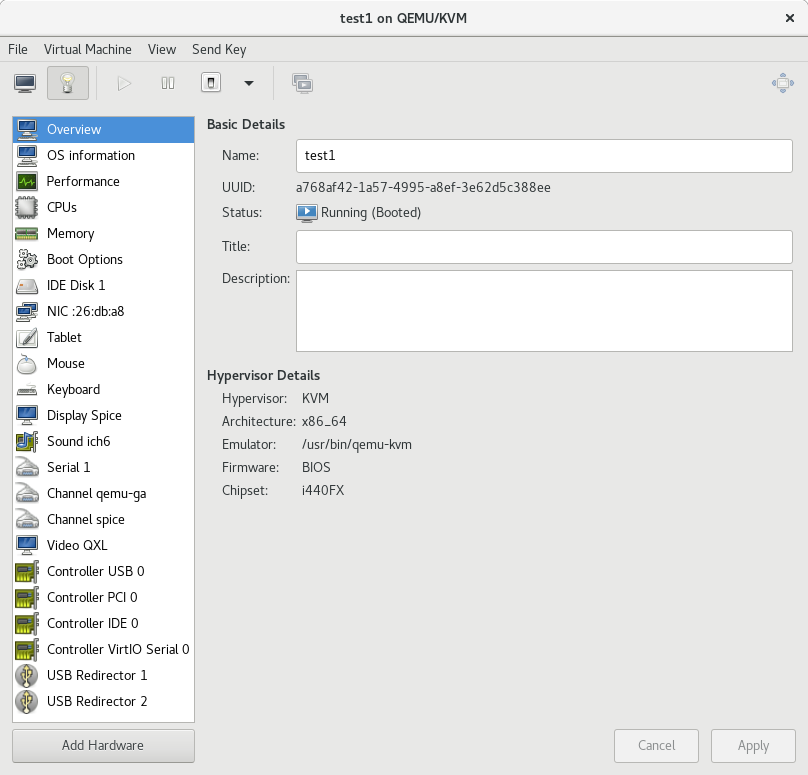
\includegraphics[height=3.2in]{IMAGES/virt-manager.png}
      \caption{virt-manager virtual hardware details}
   \end{figure}


}

\begin{frame}
   {virt-install}

	The \textbf{virt-install} is an application that uses the 
	\textbf{libvirt} interface, some of the features are: 
	\begin{itemize}
		\item command line interface 
		\item text or graphic installer interface
		\item local or network install 
		\item an import only option 
	\end{itemize}

	More information may be obtained from the associated man page or the 
	project web site, \textbf{virt-install} is part of \textbf{virt-manager} project. 
	Additional information can be found at \url{https://virt-manager.org/}.


\end{frame}

\cprotect\note{

	The \textbf{virt-install} tool adds a layer of abstraction to the 
	install process of a virtual machine. It uses \textbf{libvirt}
	 and presents the user with a command line interface. Options are
	 passed to \textbf{virt-install} describing the installation.
	 The minimum items required to start an install are: 
	 \begin{itemize}
		 \item \verb?--name?
		 \item \verb?--memory?
		 \item \verb? storage (--disk or --filesystem)?
		 \item \verb? install option (--cdrom,--location,--livecd)?
	\end{itemize}

	The example here installs from a DVD image using a text or serial 
	console. 

	\begin{raw}	
#!/bin/bash
# Sample using virt-install to install Debian from 
# DVD1 of the Debian official distribution
# Minimum disk seems to be 1.5G  
# Install contacts outside resources so a network is required. 

 virt-install \
--name test-loc \
--ram 512 \
--disk size=1.5 --vcpus 1 \
--os-type linux \
--os-variant debian9 \
--graphics none \
--boot useserial=yes  \
--cdrom /var/ftp/pub/iso/debian-9.4.0-amd64-DVD-1.iso
	\end{raw}


}


\begin{frame}
   {virt-install --import}

	The option \textbf{import} to the \textbf{virt-install} command:
	\begin{itemize}
		\item skips the install process
		\item creates a default configuration for the new VM
		\item incorporates the command line options
		\item starts the new VM in a \textbf{virt-viewer} session
	\end{itemize}

	The resulting configuration may be viewed with the \textbf{virsh dumpxml name} 
	command. 

\end{frame}

\cprotect\note{


	\begin{raw}
#!/bin/bash
# demonstrate the import function of virt-install

virt-install \
              --name import \
              --memory 512 \
              --disk /var/lib/libvirt/images/eric-x86_64.img \
	      --os-type  linux --os-variant centos6.2  \
              --import
	\end{raw}
	

	Another example of the import function, this time we 
	were given a \textbf{vmdk} disk image that used a \textbf{SCSI} 
	virtual adapter on the originating system. Unfortunately the
	initial ram disk does not have a \textbf{SCSI} driver built in.
	This is not a problem, the virtual adapter type can be changed 
	easily using the \textbf{virt-install} import with disk options:
	\begin{raw}
# virt-install  --name notscsi --memory 1024  \
	--disk path=/home/lee/Virt-KVM/CentOS7.vmdk,bus=ide \
	--ostype linux --os-variant centos7.0 \
	--import
	\end{raw} 

	The os-variant is available with the \textbf{osinfo-query os} command. 
}



